\newpage
\unappendix
\section{Smooth Manifolds}


When dealing with smooth manifolds, the idea that you want to keep in mind is that, locally, they all are supposed to look like a section of $\Rn$. As such, a good chunk of Differential Geometry deals with the ways in which we may extend our understanding of $\Rn$ to generalized differentiable manifolds. There is actually a very nice theorem (called the Whitney Embedding Theorem which will be discussed in a later section) that tells us that all smooth manifolds of dimension $n$ can be embedded in a space of dimension $\R^{2n + 1}$. But that is a topic that will not be covered until the section on Sard's Theorem. For now, we will work on how, exactly, we define smooth manifolds, and give ourselves some tools for doing Calculus on them.


\subsection{Definition of a Smooth Manifold}
\nl

\dfn We say that a topological space $M$ is a \textbf{\textit{topological n-manifold}} if 
\begin{itemize}
    \item $M$ is a Hausdorff space.
    \item $M$ is second-countable.
    \item \hl{$M$ is locally Euclidean of dimension $n$.} That is, every point $p\in M$ has a neighborhood that is homeomorphic to $\Rn$ for a fixed $n$. This means that for each $p\in M$ we can find
    \begin{itemize}
        \item an open neighborhood $U\seq M$ around $p$,
        \item an open neighborhood $\wh U\seq \Rn$, and 
        \item a homeomorphism $\vphi: U\ra \wh U$.
    \end{itemize}
\end{itemize}


\setcounter{thm}{1}

\begin{thm}[Topological Invariance of Dimension]
A non-empty topological $n$-manifold cannot be homeomorphic to a topological $m$-manifold unless $m = n$.
\end{thm}

\dfn Let $M$ be a topological $n$-manifold. A \textbf{\textit{coordinate chart}} on $M$ is an ordered pair $(U, \vphi)$, where $U$ is an open subset of $M$ (called the \textbf{\textit{coordinate domain}}) and $\vphi:U\ra \wh U$ is a homeomorphism from $U$ to an open subset $\wh U = \vphi(U) \seq \Rn$. If $\vphi(p) = 0$ for $p\in U$, then we say that the chart is \textbf{\textit{centered at p}}.

\begin{center}
    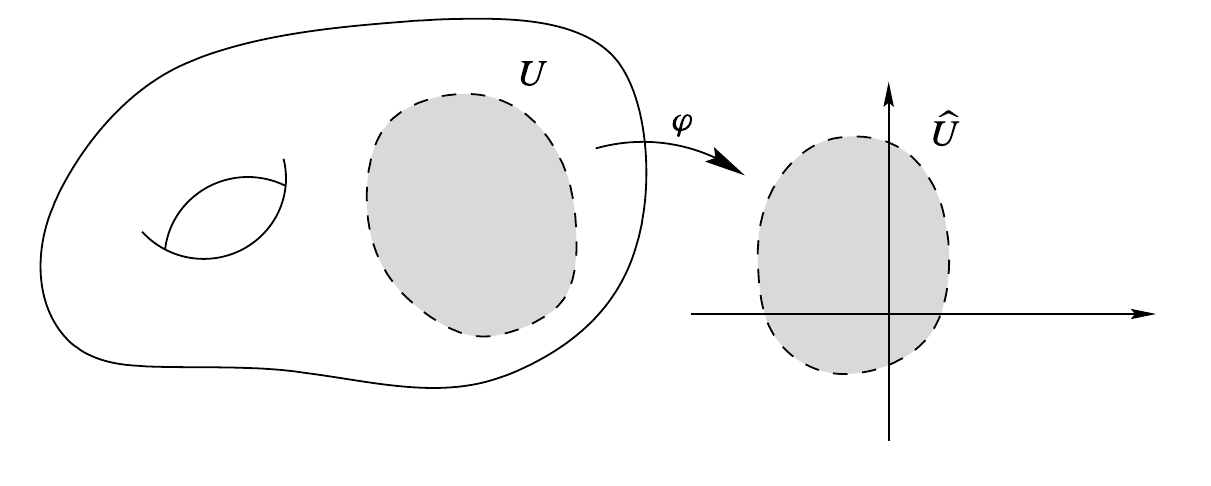
\includegraphics[scale = 0.4]{chapter01/c1f2.png}
\end{center}

\setcounter{thm}{10}

\begin{prop}
Let $M$ be a topological manifold. 
\begin{enumerate}
    \item $M$ is locally path connected.
    \item $M$ is connected if and only if it is path-connected.
    \item \hl{The components of $M$ are the same as its path components.}
    \item $M$ has countably many components, each of which is an open subset of $M$ and a connected topological manifold.
\end{enumerate}
\end{prop}

\begin{prop}
Every topological manifold is locally compact.
\end{prop}

\dfn Let $M$ be a topological space. A collection $\XX$ of subsets of $M$ is said to be \textbf{\textit{locally finite}} if each point of $M$ has a neighborhood that intersects at most finitely many members of $\XX$. 

\dfn Given a cover $\UU$ pf $M$, another cover $\VV$ is called a \textbf{\textit{refinement of $\boldsymbol{\UU}$}} if for each $V\in \VV$ there is some $U\in \UU$ such that $V\seq U$. We say that $M$ is \textbf{\textit{paracompact}} if every open cover of $M$ admits an open, locally finite refinement.

\setcounter{thm}{14}

\begin{thm}[Manifolds are Paracompact]
Every topological manifold is paracompact. In fact, given a topological manifold $M$, an open cover $\XX$ of $M$, and any basis $\BB$ for the topology on $M$, there exists a countable, locally finite open refinement of $\XX$ consisting of elements of $\BB$.
\end{thm}

\dfn If $U$ and $V$ are open subsets of Euclidean spaces $\Rn$ and $\Rm$, respectively, a function $F:U\ra V$ is said to be \hl{\textbf{\textit{smooth}}} if each of its component functions has continuous partial derivatives of all orders. If in addition $F$ is bijective and has a smooth inverse map, it is called a \hl{\textbf{\textit{diffeomorphism}}}.

\dfn Let $M$ be a topological $n$-manifold. If $(U, \vphi)$, $(V,\psi)$ are two charts such that $U\cap V\neq \es$, the composite map $\psi\circ\vphi\inv:\phi(U\cap V) \ra \psi(U\cap V)$ is called the \textbf{\textit{transition map from $\boldsymbol{\vphi}$ to $\boldsymbol{\psi}$}}. It is a composition of homeomophsims, and is therefore itself a homeomorphism. Two charts $(U,\vphi)$ and $(V,\psi)$ are said to be \textbf{\textit{smoothly compatible}} if either $U\cap V = \es$ or the transition map $\psi\circ\vphi\inv$ is a diffeomorphism.

\begin{center}
    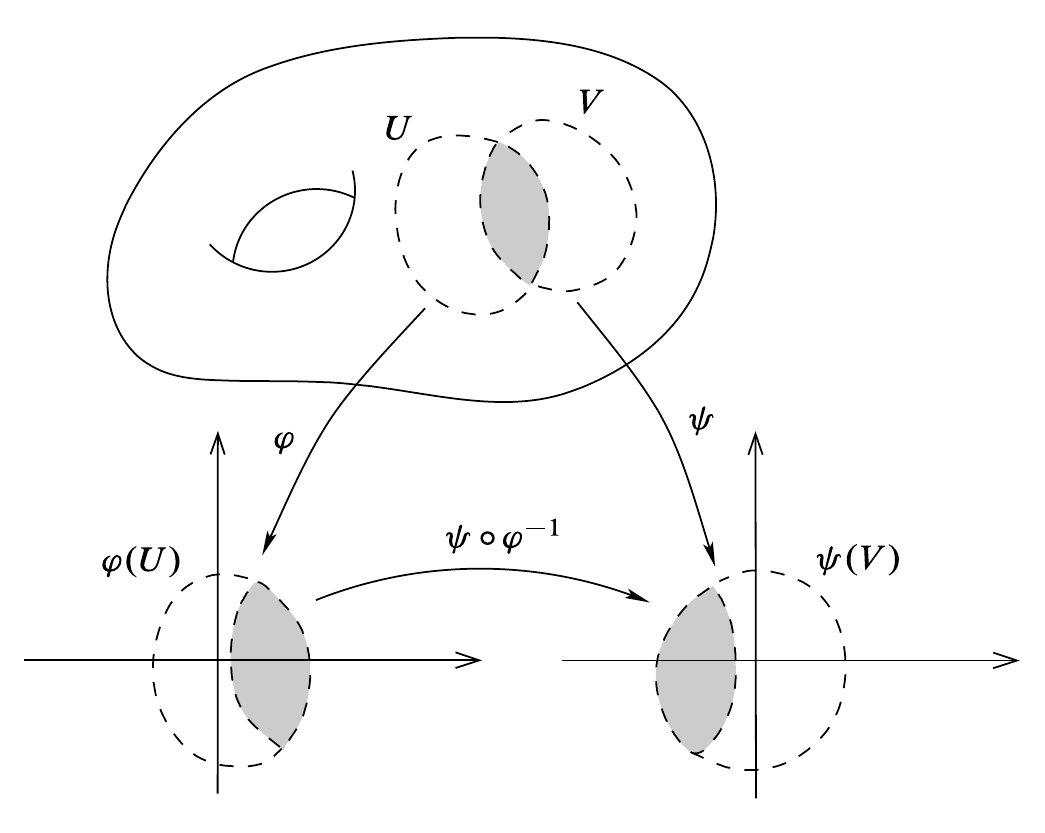
\includegraphics[scale = 0.4]{chapter01/c1f6.png}
\end{center}

\dfn An \textbf{\textit{atlas}} for a manifold $M$ is a collection of charts whose domains cover $M$. An atlas $\CA$ is called a \textbf{\textit{smooth atlas}} if any two charts in $\CA$ are smoothly compatible.

\nb Given two particular charts $(U, \vphi)$ and $(V,\psi)$, \hl{it is often easiest to show that they are smoothly compatible} by verifying that $\psi\circ\vphi\inv$ is smooth and injective with nonsingular Jacobian at each point, and appealing to Corollary C.36.

\dfn A smooth atlas $\CA$ in $M$ is \textbf{\textit{maximal}} if it is not properly contained in any larger smooth atlas. 

\dfn If $M$ is a topological manifold, a \textbf{\textit{smooth structure on M}} is a maximal smooth atlas. A \hl{\textbf{\textit{smooth manifold}}} is a pair $(M, \CA)$, where $M$ is a topological manifold and $\CA$ is a smooth structure on $M$.

\setcounter{thm}{16}

\begin{thm}Let $M$ be a topological manifold.
\begin{enumerate}
    \item Every smooth atlas $\CA$ for $M$ is contained in a unique maximal smooth atlas, called the \textbf{\textit{smooth structure determined by $\boldsymbol{\CA}$}}.
    \item Two smooth atlases for $M$ determine the same smooth structure if and only if their union is a smooth atlas.
\end{enumerate}
\end{thm}

\dfn If $M$ is a smoothm manifold, any chart $(U, \vphi)$ contained in th given maximal smooth atlas is called a \textbf{\textit{smooth chart}}, and the corresponding coordinate map $\vphi$ is called a \textbf{\textit{smooth coordinate map}}.

\subsection{Examples of Smooth Manifolds}

\setcounter{thm}{21}

\begin{ex}[Euclidean Spaces]
For each nonnegetive integer $n$, the Euclidean space $\Rn$ is a smooth $n$-manifold with the smooth structure determined by the atlas consisting of the single chart $(\Rn, \Id_\Rn)$. We call this the \textbf{\textit{standard smooth structure on $\boldsymbol{\Rn}$}} and the resulting coordinate map \textbf{\textit{standard coordinates}}. Unless we explicitly specify otherwise, we always use this smooth structure on $\Rn$. With respect to this smooth structure, the smooth coordinate charts for $\Rn$ are exactly those charts $(U,\vphi)$ such that $\vphi$ is a diffeomorphism from $U$ to another open subset $\wh U\seq \Rn$.
\end{ex}

\setcounter{thm}{24}

\begin{ex}[Spaces of Matrices]
Let $M(m\x n, \R)$ denote the set of $m\x n$ matrices with real entries. Because it is a real vector space of dimension $mn$ under matrix addition and scalar multiplication, $M(m\x n, \R)$ is a smooth $mn$-dimensional manifold. Similarly, the space $M(m\x n, \C)$ of $m\x n$ complex matrices is a vector space of dimension $2mn$ over $\R$, and thus a smooth manifold of dimension $2mn$.
\end{ex}

\begin{ex}[Open Submanifolds]
Let $U$ be any open subset of $\Rn$. Then $U$ is a topological $n$-manifold, and the single chart $(U, \Id_U)$ defines a smooth structure on $U$.

More generally, let $M$ be a smooth $n$-manifold and let $U\seq M$ be any open subset. Define an atlas on $U$ by
\[\CA_U = \{\text{smooth charts $(V, \vphi)$ for $M$ such that $V\seq U$}\}\]
Every point $p\in U$ is contained in the domain of some chart $(W, \vphi)$ for $M$; if we set $V = W\cap U$, then $(V,\vphi|_V)$ is a chart in $\CA_U$ whose domain contains $p$. It is then easy to verify that $\CA_U$ is a maximal smooth atlas for $U$, and thus any open subset of $M$ is itself a smooth $n$-manifold in a natural way. Endowed with this smooth structure, we call any open subset an \textbf{\textit{open submanifold of M}} (indeed, this will turn out to be motivation for how we define an \textit{Embedded Submanifold} later on in chapter 5).
\end{ex}

\begin{ex}[\hlo{The General Linear Group}]
The general linear group $GL(n(\R)$ is the set of $n\x n$ matrices with real entries. It is a smooth $n^2$-dimensional manifold because it is an open subset of the $n^2$-dimensional vector space $M_n(\R)$, namely the set where the (continuous) determinant function is nonzero.
\end{ex}

\setcounter{thm}{30}

\begin{ex}[Spheres]
We know that the $n$-sphere $\BSN\seq \R^{n + 1}$ is a topological $n$-manifold. We put a smooth structure on $\BSN$ as follows. For each $i = 1..n + 1$, let $(U_i^\pm. \vphi_i^\pm)$ denote the graph coordinate charts given by 
\[U_i^\pm = \{(x^1, \ldots, x^{n + 1}\in \R^{n + 1}\ :\ \pm x^i > 0\}\]
and 
\[\vphi_i^\pm (x^1,\ldots,x^{n + 1}) = (x^1,\ldots,\wh x^i,\ldots x^{n + 1}).\]
For any distinct indices $i$ and $j$, the transition map $\vphi_i^\pm\circ(\vphi^\pm)\inv$ is easily computed. In the case where $i < j$, we get 
\[\vphi_i^pm\circ(\vphi_j^\pm)\inv(u^1, \ldots, u^n) = \lp u^1,\ldots,\wh u^1,\ldots,\pm\sqrt{1 = |u|^2},\ldots,u^n\rp\]
and a similar formula holds when $i > j$. When $i = j$, $\vphi_i^+\circ(\vphi_i^-)\inv = \vphi_i^-\circ (\vphi_i^+)\inv = \Id_{\B^n}$. Thus the collection of charts $\{(\U_i^\pm, \vphi_i^\pm)\}$ is a smooth atlas, as so defines a smooth structure on $\BSN$. We call this its \textbf{\textit{standard smooth structure}}.
\end{ex}

\begin{ex}[\hlo{Level Sets}]
We can actually generalize the preceding example in the following way. Suppose $U\seq \Rn$ is an open subset and $\Phi:U\ra \R$ is a smooth function. For any $c\in \R$, the set $\Phi\inv(c)$ is called a \textbf{\textit{level set of $\boldsymbol{\Phi}$}}. Choose some $c\in \R$, let $M = \Phi\inv(c)$, and suppose it happens that the total derivative $D\Phi(a)$ is nonzero for each $a\in \Phi\inv(c)$. Because $D\Phi(a)$ is a row matrix whose entries are the partial derivatives $\lp\pd{\Phi}{x^1}(a),\ldots,\pd{\Phi}{x^n}(a)\rp$, for each $a\in M$ there is some $i$ such that $\pd{\Phi}{x^i}(a)\neq 0$. It follow from the Implicit Function Theorem, that there is a neighborhood $U_0$ of $a$ such that $M\cap U_0$ can be expressed as the graphi of an equation of the form 
\[x^i = f(x^1,\ldots,\wh x^i, \ldots, x^n),\]
for some smooth real-valued function $f$ defined on an open subset of $\R^{n - 1}$. Therefore, arguing just as in the case of the $n$-sphere, we wee that $M$ is a topological manifold of dimension $(n -1)$, and has a smooth structure such that each of the graph coordinate charts associated with a choice of $f$ as above is a smooth chart. 
\end{ex}

\begin{ex}[Projective Spaces]
The $n$-dimensional real projective space $\RPn$ is a topological $n$-manifold when given coordinate charts as in Example 1.5 of the Lee book. If we assume for convenience that $i > j$, then we can get
\[\vphi_j\circ\vphi_i\inv(u^1,\ldots,u^n) = \lp\frac{u^1}{u^j},\ldots,\frac{u^{j - 1}}{u^j},\frac{u^{j + 1}}{u^j},\ldots,\frac{u^{i - 1}}{u^j},\frac{1}{u^j},\frac{u^{i + 1}}{u^j},\ldots,\frac{u^n}{u^j}\rp,\]
which is a diffeomorphism form $\vphi_i(U_i\cap U_j)$ to $\vphi_j(U_i\cap U_j)$.
\end{ex}

\begin{ex}[Smooth Product Manifolds]
If $M_1,\ldots,M_k$ are smooth manifolds of dimensions $n_1,\ldots,n_k$, repectively, then the product space $M_1\x \cdots \x M_k$ is a topological manifold of dimension $n_1 + \cdots + n_k$, with charts of the form $(U_1\x \cdots\x U_k, \vphi_1\x \cdots \x \vphi_k)$. Any two such charts are smoothly compatible because
\[(\psi_1\x\cdots\x \psi)\circ(\vphi\x \cdots\x\vphi_k)\inv = (\psi_1\circ\vphi_1\inv)\x\cdots\x(\psi\circ\vphi_k\inv),\]
which is a smooth map. This defines a natural smooth manifold structure on the product, called the \textbf{\textit{product smooth manifold structure}}.
\end{ex}

\begin{lem}[Smooth Manifold Chart Lemma]
Let $M$ be a set, and suppose we are given a collection $\{U_\al\}$ of subsets of $M$ together with maps $\vphi_\al:U\al\ra \Rn$, such that the following properties are satisfied:
\begin{enumerate}[(i)]
    \item For each $\al, \vphi_\al$ is a bijection between $U_\al$ and an open subset $\vphi_\al(U_\al)\seq \Rn$.
    \item For each $\al$ and $\be$, the sets $\vphi_\al(U_\al\cap U_\be)$ and $\vphi_\be(U_\al\cap U_\be)$ are open in $\Rn$.
    \item Whenever $U_\al\cap U_\be \neq \es$, the map $\vphi_\be\circ\vphi_\al\inv:\vphi_\al(U_\al\cap U_\be)\ra \vphi_\be(U_\al \cap U_\be)$ is smooth,
    \item Countably many $U_\al$ cover $M$.
    \item Whenever $p,q$ are distinct points in $M$, either there exists some $U_\al$ containing both $p$ and $q$ or there exist disjoint sets $U_\al,\,U_\be$ with $p\in U_\al$ and $q\in U_\be$.
\end{enumerate}
Then $M$ has a unique smooth manifold structure such that each $(U_\al, \vphi_\al)$ is a smooth chart.
\end{lem}

\subsection{Manifolds With Boundary}
\nl

\dfn We define the \textbf{\textit{closed n-dimensional upper half-space}} $\Hn\seq \Rn$, defined as
\[\Hn = \{(x^1,\ldots, x^n)\in \Rn\ : x^n \geq 0\}.\]
We will use the notations $\Int(\Hn)$ and $\bd \Hn$ to denote the interior an boundary of $\Hn$. When $n > 0$, this means
\begin{align*}
    \Int(\Hn) &= \{(x^1,\ldots,x^n)\in \Rn\ :\ x^n > 0\},\\
    \bd\Hn &= \{(x^1,\ldots,x^n)\in \Rn\ :\ x^n = 0\}.
\end{align*}

\dfn An \textbf{\textit{n-dimensional topological manifold with boundary}} is a second-countable Hausdorff space $M$ in which every point has a neighborhood homeomorphic to either an open subset of $\Rn$ or to an open subset of $\Hn$. Charts on $M$ are defined in the obvious way, and a chart $(U,\vphi)$ will be called an \textbf{\textit{interior chart}} if $\vphi(U)$ is homeomorphic to an open subset of $\Rn$, and a \textbf{\textit{boundary chart}} if $\vphi(U)$ is homeomorphic to an open subset of $\Hn$ such that $\vphi(U)\cap \bd\Hn\neq \es$. 

\dfn A point $p\in M$ is called an \textbf{\textit{interior point of M}} if it is in the domain of some interior chart, and a \textbf{\textit{boundary point of M}} if it is in the domain of a boundary chart that sends $p$ to $\bd\Hn$.

\setcounter{thm}{37}

\begin{thm}Let $M$ be a topological $n$-manifold with boundary.
\begin{enumerate}
    \item $\Int(M)$ is an open subset of $M$ and a topological $n$-manifold without boundary.
    \item $\bd M$ is a closed subset of $M$ and a topological $(n - 1)$-manifold without boundary.
    \item $M$ is a topological manifold if and only if $\bd M = \es$.
    \item If $n = 0$, then $\bd M = 0$ and $M$ is a $0$-manifold.
\end{enumerate}
\end{thm}

\setcounter{thm}{45}

\begin{thm}[Smooth Invariance of the Boundary]
Suppose $M$ is a smooth manifold with boundary and $p\in M$. If there is some smooth chart $(U, \vphi)$ for $M$ such that $\vphi(U) \seq \Hn$ and $\vphi(p)\in \bd \Hn$, then the same is true for every smooth chart whose domain contains $p$.
\end{thm}








